\subsection{Architettura del FrontEnd}

Il funzionamento della struttura della parte Frontend si basa, appunto, sul pattern architetturale MVVM, ossia: quando l’utente esegue un’operazione nella WebApp (per esempio effettua una ricerca di un locale tramite il suo nome), il View-Model chiede al Model di scaricare i dati e/o effettuare le operazioni e rimane in attesa della risposta (nel caso di chiamate sincrone) oppure aspetta degli aggiornamenti e "osserva" (in caso di chiamate asincrone). Il Model invoca una API REST (che può essere una GET o una POST), la quale si interfaccerà con il Backend e, in caso di esito positivo, ritornerà la risposta o salverà i dati (in base all'operazione effettuata). \\
Una volta che il Model avrà finito l'operazione, ritornerà direttamente la risposta al View-Model nei casi in cui è necessaria oppure notificherà il View-Model che i dati "osservati" sono cambiati, il quale, allora, chiederà al Model di restituirgli i dati aggiornati. Successivamente, quando anche i dati del View-Model sono stati aggiornati, anche la View riceverà una notifica, stavolta del View-Model, che gli chiederà di re-renderizzarsi con i nuovi dati aggiornati. 



\begin{figure}[H]
    \centering
    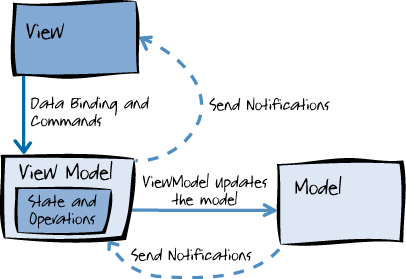
\includegraphics[scale=0.5]{Contenuto/Immagini/MVVM.png}
    \caption{Schema MVVM}
\end{figure}

In questo modo si ha una netta separazione tra chi salva ed elabora i dati (il Model) e chi li mostra (la View), mentre il View-Model funge da tramite tra le due parti. 
In accordo con il proponente, per realizzare la parte Frontend della WebApp, abbiamo scelto di utilizzare la libreria JavaScript React, per la quale viene fornita un'integrazione del meccanismo degli observer tramite la libreria \textit{MobX} (che abbiamo deciso di adottare per alcune componenti del nostro progetto).


RIMUOVERE!?
In particolar modo, abbiamo implementato gli observer in alcune parti della:
\begin{itemize}
\item View, perché attende di aggiornarsi quando l’utente interagisce con la WebApp (p.es. sfruttiamo gli observer quanto l'utente effettua una ricerca o clicca su dei bottoni, operazioni tramite le quali l'utente si aspetta di ricevere qualcosa),
\item View-Model, perché questa parte rimane in attesa di ricevere una promise da parte del Model in merito alla “bontà” dell’operazione richiesta (nel caso l’operazione abbia esito positivo, vengono ritornati i dati da renderizzare nella View, altrimenti verrà ritornato un errore).
\end{itemize}
RIMUOVERE!?
